\subsection{Forward error correcting}

In telecommunications and computing, forward error correction (FEC) is a digital signal processing technique used to control errors in data transmission over unreliable or noisy communication channels, as well as to independently increase data reliability at the receiver to ensure high quality.

FEC improves bit error rate efficiency in communication systems, but involves additional digital processing, making it more expensive in terms of cost and spectral efficiency. The balance between these two elements needs to be taken into account in systems.

This is achieved by introducing redundant data using error-correcting codes (ECC) before the message is transmitted.  Without redundancy, every piece of data in the message is essential to its understanding. Any error in the message can therefore change its meaning.  The aim is to ensure that errors do not compromise the overall understanding of the message, and do not trigger a request for a re-transmission of the message by the receiver, thereby reducing channel traffic by more than a factor of two.

\subsubsection{Introduction to error correction code}

The problems encountered by modern industry are very diverse, all offering multiple techniques used for error-correcting codes. In some cases, such as data transmission over the Internet, the ECC's role is limited to error detection. In other cases, such as the TCP protocol on the transport layer of the OSI model, when an error is detected during message transmission, it is corrected by retransmitting the message. The techniques listed here are just a few of a sea of others, and today we're going to take a look at a very special technique known for its effectiveness : \textbf{Convolutional correctors}

The special feature of a convolutional ECC is that its output depends on the current symbol to be coded, as well as the previous symbol and the result of coding the previous symbol, unlike block codes, which process each block of information independently of the others.

For the purposes of this report, we will confine ourselves to the case of discrete communication channels, which are nothing other than binary channels transmitting only 0 or 1, i.e. bits of information.

\subsubsection{Convolutional encoding}

\begin{figure}[H]
    \centering
    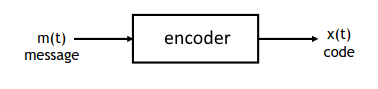
\includegraphics[width=0.5\linewidth]{images/encodeur_schem.png}
    \caption{Communication encoder diagram}
    \label{fig:encoder-diagram}
\end{figure}

A convolutional encoder is a finite state machine, and its state diagram can be represented as a lattice (the temporal equivalent of a state diagram). All states are arranged in columns to represent a state at time \textbf{t}, where \textbf{m(t)} and \textbf{x(t)} are discrete signals whose samples are binary. These states are linked to the same sets of states representing time t+1, in accordance with the transition table.

\begin{figure}[H]
    \centering
    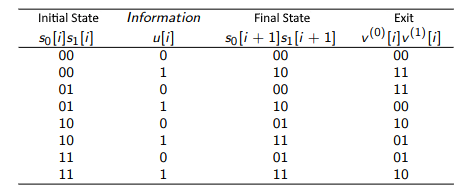
\includegraphics[width=0.5\linewidth]{images/transitionTable.png}
    \caption{Transition table with i for the clock time}
    \label{fig:transition-table}
\end{figure}

If the encoder is a linear system, \textbf{x(t)} can be generated by a convolution product:
\[ x_{j} = \sum_{i=0}^M g_{i}m_{j-i} \]

In order to carry out a binary convolution coding we will set some parameters:
\begin{itemize}
     \item $g_{i} = 0 \rightarrow$ connection absent
     \item $g_{i} = 1 \rightarrow$ connection present
     \item $K \rightarrow$ Constraint length (number of sampling instants during which a message bit participates in the elaboration of the output)
\end{itemize}

This is a so-called sliding window coding where there are two integers \textit{m} (for memory) and \textit{a} (for anticipation) such that the index symbol n of the coded sequence depends only on the finite source block between the indices $n - m$ and $n + a$.
\begin{figure}[H]
    \centering
    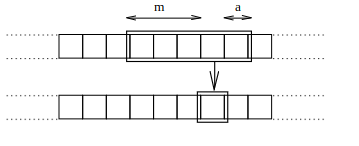
\includegraphics[width=0.5\linewidth]{images/register.png}
    \caption{Shift register}
    \label{fig:shift-register}
\end{figure}

For 1/2-rate 2-memory convolutional encoder we take M = 2, then we have K = M + 1 = 3 with an output interleaving n = 2, so using the above formula we obtain the following generator polynomials: $g_{1} = [1, 1, 1]$ and $g_{2} = [1, 0, 1]$.

All these parameters allow us to obtain the following logic diagram, enabling convolutional coding of our ECC: 
\begin{figure}[H]
     \centering
     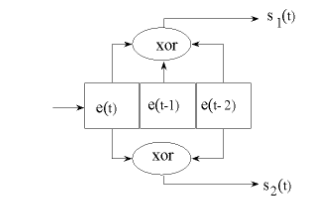
\includegraphics[width=0.5\linewidth]{images/logical_circuit.png}
     \caption{Data transmission in a convolutional encoder with a shift register and exclusive ORs}
     \label{fig:logical-circuit}
\end{figure}

Using this schema and XORing according to the connections said to be absent or present on the register undergoing a shift along the chain to be encoded we obtain:
\begin{itemize}
 \item Initial string : \textbf{1010}
 \item Encoded string: \textbf{11100010}
\end{itemize}

We therefore observe the presence of redundancy, as explained in the introduction, with a redundancy bit for each bit of the initial character string, which we'll use for decoding.

Before we start decoding, as we are working on noisy discrete channels, we will apply noise to the character string to check that our appended code is working correctly. Our message therefore becomes $\rightarrow$ \textbf{11100011}


\subsubsection{Decoding with Viterbi algorithm}

The Viterbi algorithm is based on the dynamic programming paradigm. We start from a starting state (default 00) and seek to find the path from the starting state whose output has the same length and is as close as possible to the message to be decoded. To apply this notion of proximity, we use the Hamming distance, which counts the number of different bits between two messages of the same finite or infinite length. 

This Hamming distance can be translated into the following pseudo-code:

\begin{algorithm}[H]
\begin{algorithmic}
\Function{Hamming distance}{$\text{s1}, \text{s2}$}
    \If{$\text{len}(\text{s1}) \neq \text{len}(\text{s2})$}
        \State \Return "Strings must be of equal length"
    \EndIf
    \State $\text{dist} \gets 0$
    \For{$i \gets 0$ \textbf{to} $\text{len}(\text{s1}) - 1$}
        \If{$\text{s1}[i] \neq \text{s2}[i]$}
            \State $\text{dist} \gets \text{dist} + 1$
        \EndIf
    \EndFor
    \State \Return $\text{dist}$
\EndFunction
\end{algorithmic}
\end{algorithm}

In response to the dynamic programming paradigm, the Viterbi algorithm can be represented in ways other than as a lattice. For the sake of simplicity, it will be presented in the form of a binary tree, so that we can create a history of all possible paths and perform a recursion to calculate the metric of each path from that of each branch, and reconstruct the message to be decoded.

\begin{figure}[H]
     \centering
     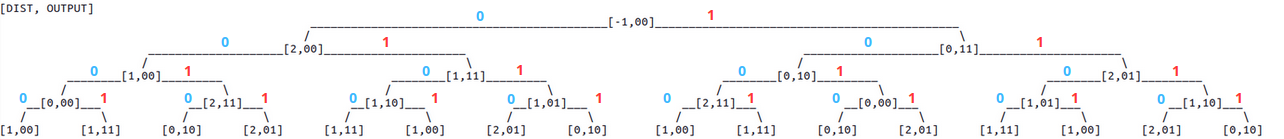
\includegraphics[width=1\linewidth]{images/BT_ECC_CV.png}
     \caption{Representation of the binary tree of the Viterbi lattice}
     \label{fig:bt-ecc-cv}
\end{figure}

Using the transition table in figure n°\ref{fig:transition-table}, we can move from one state to another and retrieve the new state, as well as the output bits, all thanks to the input bits which are 0 for the nodes on the left and 1 for the nodes on the right. A state is in fact a pair of bits resulting from the concatenation of the initial bit and the redundancy bit. If we go back up our tree, all we have to do is concatenate the input bits to reconstitute the message, even if it has been noisy. We know which is the safest path to take thanks to the distances noted above.

\begin{figure}[H]
     \centering
     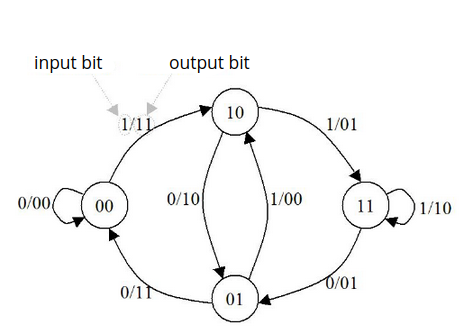
\includegraphics[width=0.5\linewidth]{images/logical_circuit_v2.png}
     \caption{State diagram of a convolutional encoder with 2 memories and 1/2 rate}
     \label{fig:logical_circuit_v2}
\end{figure}

Now, we can retrieve the correct message that is \textbf{1010}.

\newpage